\usetikzlibrary{calc,positioning}
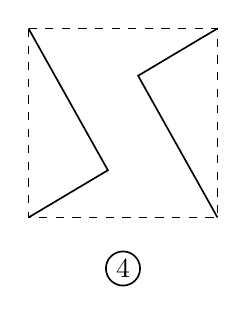
\begin{tikzpicture}[x=2.4cm,y=2.4cm,line width=.6pt,font=\normalsize]
% Option (4): dashed unit square (a face of the cube) with two separated solid polylines,
% centrally symmetric, endpoints on the square corners; label circleded 4 below.
\coordinate (TL) at (0,1);
\coordinate (TR) at (1,1);
\coordinate (BL) at (0,0);
\coordinate (BR) at (1,0);
\coordinate (P1) at (0.42,0.25);
\coordinate (P2) at (0.58,0.75);
\draw[line width=.6pt,dashed] (TL) -- (TR) -- (BR) -- (BL) -- cycle;
\draw[line width=.6pt] (TL) -- (P1) -- (BL);
\draw[line width=.6pt] (TR) -- (P2) -- (BR);
\node[draw,circle,line width=.6pt,inner sep=1.5pt] at (0.5,-0.27) {$4$};
\end{tikzpicture}
